\chapter{机器学习概述与数据特征工程}
\section{引言}


\section{名字还没取号呢}
\subsection{机器学习概述}

计算机程序利用经验$E$学习任务$T$,性能是$P$,如果针对任务$T$的性能$P$随着经验$E$不断增长,则称为机器学习。
\begin{figure}[htbp]
  \centering
  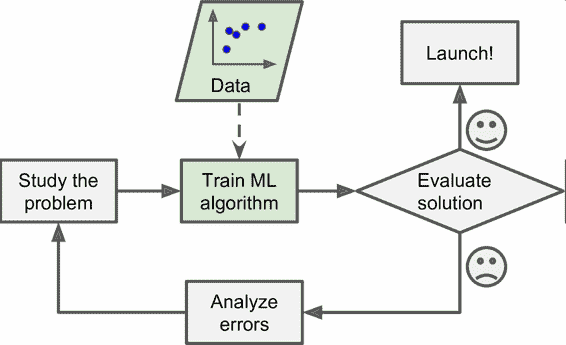
\includegraphics[width=.6\linewidth]{features/ml}
  \caption[机器学习方法]{\label{fig:ml}机器学习方法\cite{Aurélien2018}}
\end{figure}

\subsection{机器学习的一般步骤}

* 提出具体问题(PE甄别)
* 获取数据(原始PPG->特征提取)
* 研究数据的特性(相关性、有效性,分布特性)
* 数据准备(缺失值、标准化、特征筛选、构建新特征等)
* 探索多种机器学习模型,列出最佳模型
* 超参数调整,优化最佳模型
* 结论与演示,什么有效什么无效,最后结果
* 生产与部署

\subsection{本研究的机器学习目标}
探求子痫前期与脉搏波波形之间的潜在关系,

探求子痫前期与孕妇脉搏波数据之间的关系


\section{数据特征工程}
特征的处理

\subsection{数据集构建}
* 分析数据集准备:两种方式

  * A. by pulse

  * B. by person
\subsection{PPG时域描述特征集构建}

本小节对本研究实际采用的多种PPG时域描述特征进行汇总,对各参数符号及前置计算条件也进行了统一说明,如\autoref{tab:allfeatures}所示。
TODO
\begin{center}
    \fontsize{10}{4}
    \begin{longtable}{p{3cm}<{\centering}p{1cm}<{\centering}p{2cm}<{\centering}p{6cm}<{\centering}p{1cm}<{\centering}}
        \caption{本研究使用的所有PPG时域指标一览}\\
        \label{tab:allfeatures}\\
        \hline\hline
            \textbf{研究者}&\textbf{时间}&\textbf{脉搏波参数}&\textbf{研究结果}&\textbf{备注}\\
        \hline
        \endfirsthead
        \caption[]{(续)}\\
        \hline
            \textbf{研究者}&\textbf{时间}&\textbf{脉搏波参数}&\textbf{研究结果}&\textbf{备注}\\
        \hline
        \endhead 
        \hline
        \endfoot
        \hline\hline
        \endlastfoot
        &       &       &       &  \\
        &       &       &       &  \\
        &       &       &       &  \\
        &       &       &       &  \\
        &       &       &       &  \\
    \end{longtable}
\end{center}
\subsection{两种划分方式}
\subsection{数据集的处理}

\section{数据清洗}
* 处理缺失值

\section{新特征的创建}
* 构建新特征(char参数)
\section{相关性验证}
* 分布特性

  * 有无差异性,SPSS统计,已用python实现

  * 特征相关性,heatmap
\section{特征缩放}
* 标准化
\section{特征降维}
* 降维与特征贡献度

* 部分工作需要下一章节完成后才能确认
\section{小结}